\documentclass{article}
\usepackage{tikz}
\usetikzlibrary{shapes.geometric,calc,angles,positioning,intersections,quotes,decorations,babel,patterns,fit}
\usepackage{tkz-euclide}
\begin{document}
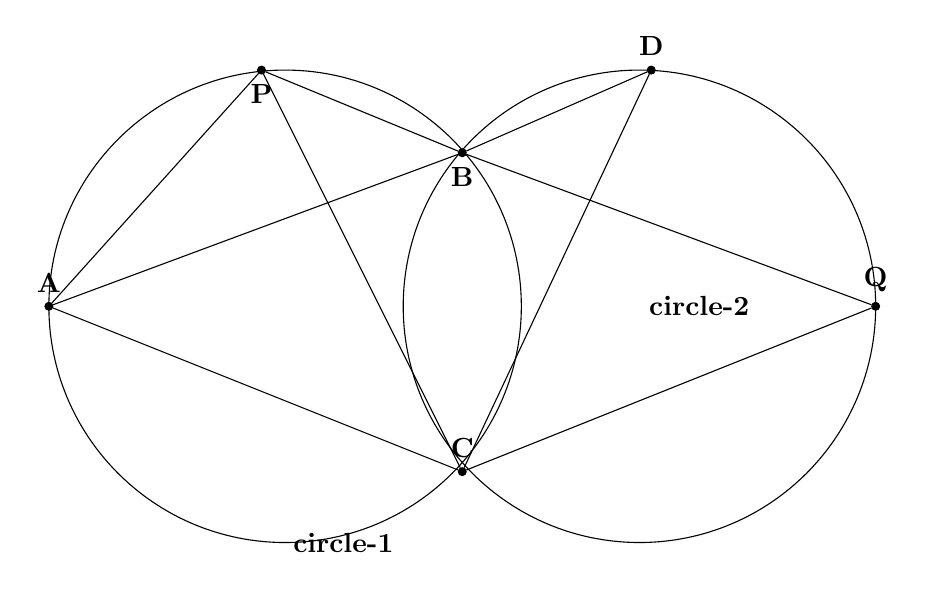
\begin{tikzpicture}[scale =1.5,>=stealth,point/.style = {draw, circle, fill = black, inner sep = 1pt},]
\draw node[left] {$\textbf{circle-1}$}(2,2)circle (2cm)node[right] {$\textbf{circle-2}$} (-1,2) circle (2cm);
\node (A) at (-3,2)[point,label=above :$\textbf{A}$] {};
\node (P) at (-1.2,4)[point,label=below :$\textbf{P}$] {};
\node (B) at (0.5,3.3)[point,label=below :$\textbf{B}$] {};
\node (Q) at (4,2)[point,label=above :$\textbf{Q}$] {};
\node (D) at (2.1,4)[point,label=above :$\textbf{D}$] {};
\node (C) at (0.5,0.6)[point,label=above :$\textbf{C}$] {};
\draw (A)--(P)--(B)--(Q)--(C)--(P);
\draw (A)--(B)--(D)--(C)--(A);
\end{tikzpicture}
\end{document}